\chapter{玻尔兹曼因子}\label{ch:b2:boltzmann-factor}

登上山峰，空气便稀薄起来：在三千米高处，
气压已降至 \qty{0.7}{bar}，在珠穆朗玛峰顶则降为
海平面值的三分之一。大气上方没有任何东西约束它；它
靠引力聚拢、靠热运动散开，二者折中的结果是一个指数，
即 $n \propto
\eu^{-mgz/k_BT}$ ——分子势能与
$k_BT$ 之比决定了它在高处有多稀薄。同一指数函数支配着
激发能级上原子所占的比例、速度足够快以逃离
行星的分子数、顺磁体的磁化强度、
激光器必须反转的粒子数，以及普朗克定律所计数的
量子：它就是\emph{玻尔兹曼因子}，统计物理学中最有用的
公式。本章先由大气层引入它，
再给出一般表述，并仅用求和与高斯积分，
由它导出两能级系统及其热容、
能量均分定理、分子速率分布，
以及顺磁性的居里定律——途中还将给出
量子振子的平均能量，即普朗克公式。

\begin{omfigure}
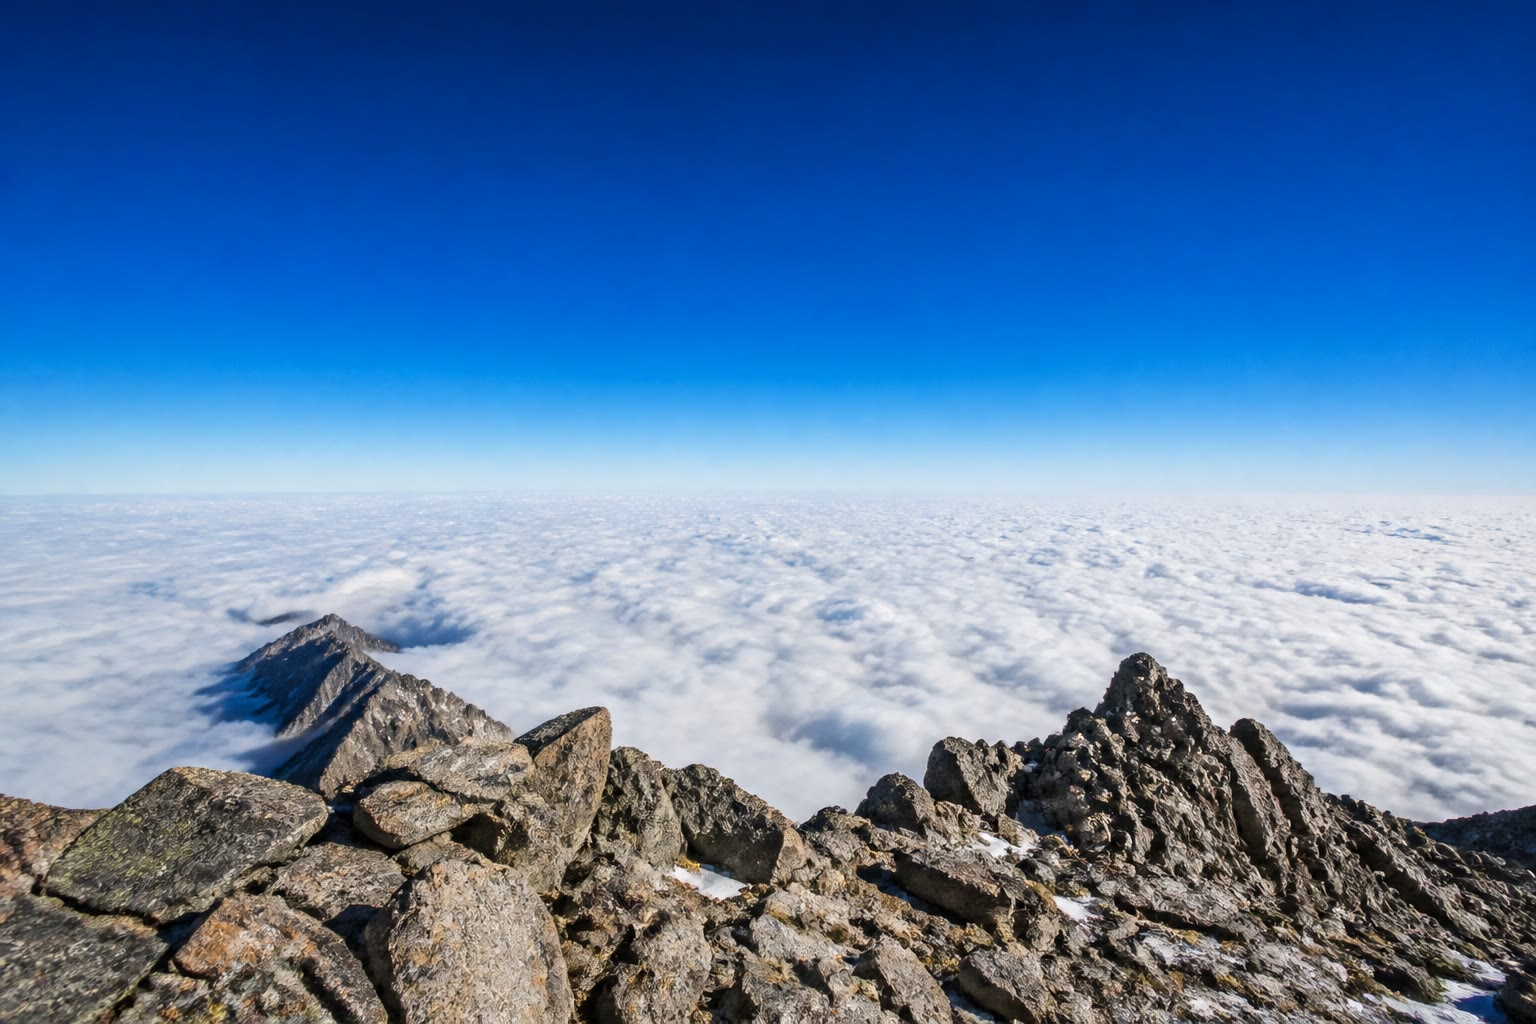
\includegraphics[width=0.58\linewidth]{images/book4/ai/b4-29-sky-gradient-summit.jpg}

{\small 自山顶望去，下层大气的雾霭与上方的深蓝天空：
空气密度每升高 \qty{8}{km} 便减小一个因子 $\eu$，
这正是分子在地球引力场中势能的
玻尔兹曼因子。}
\end{omfigure}

\section{等温大气}

\begin{proposition}[气压定律]\label{prop:b2:boltzmann-factor:barometric}
设分子质量为 $m$ 的理想气体大气，处于均匀
温度 $T$、均匀重力场 $g$ 中，压强与数密度
随高度按指数规律减小：
\[
P(z) = P_0\,\eu^{-z/H}, \qquad n(z) = n_0\,\eu^{-mgz/k_BT}, \qquad
H = \frac{k_BT}{mg} ,
\]
其中\emph{标高}\index{标高} $H \approx \qty{8.4}{km}$（温度为
\qty{288}{K} 的空气）。指数为分子势能
$mgz$ 与热能 $k_BT$ 之比。
\end{proposition}

\begin{proof}
由流体静力学 $\dd P/\dd z = -\rho g = -nmg$，并结合理想气体定律 $P
= nk_BT$，得 $\dd P/\dd z = -(mg/k_BT)P$，是一个指数函数。真实
大气随高度降温（最低十
千米内约为 \qty{6.5}{K/km}），使下降略快；等温模型
的近似精度约为 $20\%$。
\end{proof}

\begin{omfigure}
\begin{tikzpicture}
  \begin{axis}[omaxis, width=8.2cm, height=4.8cm, xmin=0, xmax=32, ymin=0, ymax=1.1,
    xlabel={$z$（\unit{km}）}, ylabel={$P/P_0$}, xtick={8.4,16.8,25.2}, xticklabels={$H$,$2H$,$3H$}, ytick={0.37,1}, yticklabels={$1/\eu$,$1$}, clip=false,
    legend style={font=\scriptsize, at={(0.97,0.45)}, anchor=north east, draw=none, fill=none}]
    \addplot[omDef, thick, domain=0:32, samples=80] {exp(-x/8.4)};
    \addlegendentry{空气，\qty{288}{K}}
    \addplot[omExo, thick, dashed, domain=0:32, samples=80] {exp(-x/60)};
    \addlegendentry{仅氦气，$H = \qty{60}{km}$}
    \draw[dashed, gray] (axis cs:8.4,0) -- (axis cs:8.4,0.37) -- (axis cs:0,0.37);
  \end{axis}
\end{tikzpicture}

{\small 等温大气：压强与密度每经过一个标高，便降为原来的 $1/\eu$
倍，标高 $H = k_BT/mg$；较轻的气体将具有更大的 $H$
——但在 \qty{100}{km} 以下，湍流使空气保持混合，所有
气体共享平均标高 $H$。}
\end{omfigure}

\section{玻尔兹曼因子}

\begin{theorem}[玻尔兹曼因子]\label{thm:b2:boltzmann-factor:factor}
与热源达成热平衡、温度为
$T$ 的系统，处于能量为 $E$ 的某一微观态的
概率正比于
\[
\eu^{-E/k_BT} .
\]
于是，对能量为 $E_i$ 的一组离散态，
\[
p_i = \frac{\eu^{-E_i/k_BT}}{Z}, \qquad Z = \sum_i\eu^{-E_i/k_BT} ,
\]
和 $Z$（\emph{配分函数}\index{配分函数}）
用于归一化各概率；两个态（或两个简并度相同的
能级）的粒子数之比为 $N_2/N_1 = \eu^{-(E_2 - E_1)/k_BT}$；
而对连续变量（如位置、速度），概率
密度关于该变量正比于 $\eu^{-E/k_BT}$。在
\qty{300}{K} 时，$k_BT = \qty{4.1e-21}{J} = \qty{0.026}{eV}$：凡
代价远高于此的状态很罕见，代价远低于此的
则很容易被激发。
\end{theorem}

\begin{proof}
气压定律即为势能 $mgz$ 所对应的因子；
其一般性在本阶段不加证明地承认，但这里给出论证（严格化见
本科三年级分册）。热源 $R$ 很大；当小系统处于
能量为 $E$ 的状态时，热源的能量为 $E_{\text{tot}} -
E$，可处于 $\Omega_R(E_{\text{tot}} - E)$ 个微观态，它们
等概率（孤立整体的基本假设）。于是
$p(E) \propto \Omega_R(E_{\text{tot}} - E)$。由玻尔兹曼的
熵的定义 $S_R = k_B\ln\Omega_R$，对热源有 $1/T = \dd S_R/\dd E_R$，
即热源的 $\ln\Omega_R(E_{\text{tot}} - E) \approx \ln\Omega_R(E_{\text{tot}})
- E/k_BT$，因为 $E \ll E_{\text{tot}}$；取指数。
\end{proof}

\begin{example}[原子能级的粒子数]\label{ex:b2:boltzmann-factor:levels}
氢原子的第一激发能级比基态高
\qty{10.2}{eV}。在 \qty{300}{K} 时，$\eu^{-395}$ ——宇宙中找不到一个这样的原子；在
\qty{6000}{K}（太阳表面）时，$\eu^{-19.7} \approx 3 \times 10^{-9}$（乘以
简并度 $4$）：这足以使太阳巨大的气柱中出现
巴耳末吸收线，它在 \qty{10000}{K} 左右的恒星中最强。
钠的 D 线（\qty{2.1}{eV}）出现在 \qty{2500}{K} 的火焰中：$\eu^{-9.8} = 6
\times 10^{-5}$ 的原子被激发，由此产生
了一小撮食盐的黄色火焰。而\cref{ch:b2:laser}所讨论的激光介质中，
该因子表明其上能级在平衡时是空的，泵必须
与之对抗。
\end{example}

\section{离散能级：两能级系统与振子}

\begin{proposition}[配分函数给出的平均能量]\label{prop:b2:boltzmann-factor:meanE}
记 $\beta = 1/k_BT$，
\[
\langle E\rangle = \sum_ip_iE_i = -\frac{\partial\ln Z}{\partial\beta}, \qquad
C = \frac{\dd\langle E\rangle}{\dd T} .
\]
\end{proposition}

\begin{proof}
$\partial_\beta Z = -\sum E_i\eu^{-\beta E_i}$，除以 $Z$。
\end{proof}

\begin{proposition}[两能级系统]\label{prop:b2:boltzmann-factor:twolevel}
$N$ 个相互独立的系统，各有两个能级 $0$ 与 $\varepsilon$（磁场中的
自旋、有一个激发能级的原子、有两个位置的缺陷）：
\[
\frac{N_2}{N} = \frac{1}{\eu^{\varepsilon/k_BT} + 1}, \qquad
\langle E\rangle = \frac{N\varepsilon}{\eu^{\varepsilon/k_BT} + 1}, \qquad
C = Nk_B\,\frac{x^2\eu^x}{(\eu^x + 1)^2}, \quad x = \frac{\varepsilon}{k_BT} .
\]
低温时上能级为空，高温时至多半满，
（平衡时从不反转）；热容
两端为零，峰值为 $0.44\,Nk_B$，出现在 $k_BT = 0.42
\varepsilon$ 附近——\emph{肖特基反常}\index{肖特基反常}，
即能谱中存在能隙的标志。
\end{proposition}

\begin{proof}
$Z = 1 + \eu^{-x}$；$p_2 = \eu^{-x}/(1 + \eu^{-x})$；对 $\langle
E\rangle$ 关于 $T$ 求导。
\end{proof}

\begin{omfigure}
\begin{tikzpicture}
  \begin{axis}[omaxis, width=6.4cm, height=4.4cm, xmin=0, xmax=3.2, ymin=0, ymax=1.1,
    xlabel={$k_BT/\varepsilon$}, ylabel={布居数}, xtick={1,2,3}, ytick={0.5,1}, clip=false]
    \addplot[omDef, thick, domain=0.02:3.2, samples=100] {1/(exp(1/x)+1)};
    \addplot[omExo, thick, domain=0.02:3.2, samples=100] {exp(1/x)/(exp(1/x)+1)};
    \node[font=\scriptsize, omExo] at (axis cs:1.4,0.85) {$N_1/N$};
    \node[font=\scriptsize, omDef] at (axis cs:1.4,0.2) {$N_2/N$};
  \end{axis}
  \begin{axis}[omaxis, width=6.4cm, height=4.4cm, xmin=0, xmax=3.2, ymin=0, ymax=0.55, xshift=6.6cm,
    xlabel={$k_BT/\varepsilon$}, ylabel={$C/Nk_B$}, xtick={1,2,3}, ytick={0.44}, clip=false]
    \addplot[omThm, thick, domain=0.08:3.2, samples=120] {(1/x)^2*exp(1/x)/(exp(1/x)+1)^2};
    \draw[dashed, gray] (axis cs:0.42,0) -- (axis cs:0.42,0.44);
    \node[font=\scriptsize, below] at (axis cs:0.42,0) {$0.42$};
  \end{axis}
\end{tikzpicture}

{\small 两能级系统：布居数随温度的变化（上能级
逐渐趋向一半，但从不超过一半）与肖特基热容，
即 $k_BT$ 与能隙相当时出现的凸起。}
\end{omfigure}

\begin{proposition}[量子振子与普朗克公式]\label{prop:b2:boltzmann-factor:oscillator}
频率为 $\nu$ 的谐振子具有能级 $E_n = nh\nu$（可再加
一个常数）；温度为 $T$ 时，
\[
Z = \frac{1}{1 - \eu^{-h\nu/k_BT}}, \qquad
\langle E\rangle = \frac{h\nu}{\eu^{h\nu/k_BT} - 1}
\ \longrightarrow\
\begin{cases} k_BT & (h\nu \ll k_BT), \\ h\nu\,\eu^{-h\nu/k_BT} & (h\nu \gg k_BT). \end{cases}
\]
这就是辐射场某一模式的平均能量，普朗克
定律（见\cref{ch:b2:thermal-radiation}）将其乘以模式数，
也是固体中振动的平均能量：高温时为
经典的 $k_BT$；低温时则为冻结的模式。
\end{proposition}

\begin{proof}
等比级数求和，再求 $-\partial_\beta\ln Z$。
\end{proof}

\begin{example}[固体的热容]\label{ex:b2:boltzmann-factor:einstein}
将固体中每个原子看作三个频率相同的振子
$\nu$（爱因斯坦，1907 年）：$C = 3Nk_B\,x^2\eu^x/(\eu^x - 1)^2$，其中 $x =
h\nu/k_BT$。温度高于 $\theta_{\text{E}} = h\nu/k_B$ 时，$C \to 3Nk_B = 3R$（每摩尔）
——即杜隆–珀蒂定律（\qty{25}{J/mol/K}），铅、
铜、铁在室温下都符合；远低于此温度时，$C$ 骤降。
金刚石（$\theta_{\text{E}} \approx \qty{1300}{K}$）在
\qty{300}{K} 时仅为 \qty{6}{J/mol/K}，经典物理无法解释，而每种固体的热容
在低温下都趋于零——这是量子理论在辐射之外的
第一个成功。
\end{example}

\section{能量均分与麦克斯韦分布}

\begin{theorem}[能量均分定理]\label{thm:b2:boltzmann-factor:equipartition}
凡以二次形式进入能量的变量 $q$，$E = aq^2 +
\dots$，且取遍全体实数，在平衡态下对
平均能量的贡献为 $\tfrac12k_BT$：
\[
\langle aq^2\rangle = \tfrac12k_BT .
\]
单原子气体（三个平动）有 $U = \tfrac32Nk_BT$，且 $C_V =
\tfrac32R$（每摩尔）；双原子气体增加两个转动，$C_V = \tfrac52R$，
而其振动（两个二次项，但因量子化而有 $h\nu \gg
k_BT$，在室温下仍被冻结，直到几千开尔文。
\end{theorem}

\begin{proof}
关于 $q$ 的概率密度为 $\propto\eu^{-aq^2/k_BT}$，即高斯分布：
\[
\langle aq^2\rangle = \frac{\int aq^2\,\eu^{-aq^2/k_BT}\,\dd q}{\int\eu^{-aq^2/k_BT}\,\dd q} = \tfrac12k_BT
\]
（将 $\int\eu^{-\lambda q^2}\dd q = \sqrt{\pi/\lambda}$ 对
$\lambda$ 求导）。该结果要求能级连续：当
相邻能级的间距大于 $k_BT$ 时，该因子使该变量冻结，
与前面的振子情形一样。
\end{proof}

\begin{theorem}[麦克斯韦速率分布]\label{thm:b2:boltzmann-factor:maxwell}
在温度为 $T$ 的气体中，速度分量是
方差为 $k_BT/m$ 的独立高斯分布，速率 $v = |\vect v|$ 的
概率密度为
\[
f(v) = 4\pi\Big(\frac{m}{2\pi k_BT}\Big)^{3/2}v^2\,\eu^{-mv^2/2k_BT} ,
\]
最可几速率、平均速率和方均根速率分别为
\[
v_{\text{p}} = \sqrt{\frac{2k_BT}{m}}, \qquad
\langle v\rangle = \sqrt{\frac{8k_BT}{\pi m}}, \qquad
v_{\text{rms}} = \sqrt{\frac{3k_BT}{m}} ,
\]
三者之比为 $1 : 1.13 : 1.22$。\qty{300}{K} 下的氮气为 \qty{422}{}，
\qty{476}{}，\qty{517}{m/s}；氢气则为其 $3.7$ 倍；分布的
尾部 $\propto\eu^{-mv^2/2k_BT}$ 使
最快的分子得以蒸发、发生反应，或脱离行星。
\end{theorem}

\begin{proof}
动能 $\tfrac12m(v_x^2 + v_y^2 + v_z^2)$ 给出因子
$\eu^{-mv_x^2/2k_BT}\eu^{-mv_y^2/2k_BT}\eu^{-mv_z^2/2k_BT}$：三个独立的
高斯函数，各自由 $\sqrt{m/2\pi k_BT}$ 归一化。速率
分布是将半径为 $v$ 的球壳内的全部速度汇总，
其体积为 $4\pi v^2\dd v$。$v_{\text{p}}$ 由 $\dd f/\dd v = 0$ 得出，而各阶矩
由 $\int_0^\infty v^3\eu^{-av^2}\dd v = 1/2a^2$、$\int_0^\infty
v^4\eu^{-av^2}\dd v = \tfrac38\sqrt{\pi/a^5}$ 求得；$v_{\text{rms}}$ 也可由能量均分定理得出，
$\tfrac12m\langle v^2\rangle = \tfrac32k_BT$。
\end{proof}

\begin{omfigure}
\begin{tikzpicture}
  \begin{axis}[omaxis, width=9cm, height=5cm, xmin=0, xmax=1750, ymin=0, ymax=0.0028,
    xlabel={$v$ (\unit{m/s})}, ylabel={$f(v)$}, xtick={400,800,1200}, ytick=\empty, clip=false,
    legend style={font=\scriptsize, at={(0.97,0.95)}, anchor=north east, draw=none, fill=none}]
    \addplot[omDef, thick, domain=0:1600, samples=160] {4*pi*(28*1.66e-27/(2*pi*1.38e-23*100))^1.5*x^2*exp(-28*1.66e-27*x^2/(2*1.38e-23*100))};
    \addlegendentry{N$_2$, \qty{100}{K}}
    \addplot[omThm, thick, domain=0:1600, samples=160] {4*pi*(28*1.66e-27/(2*pi*1.38e-23*300))^1.5*x^2*exp(-28*1.66e-27*x^2/(2*1.38e-23*300))};
    \addlegendentry{N$_2$, \qty{300}{K}}
    \addplot[omExo, thick, domain=0:1600, samples=160] {4*pi*(28*1.66e-27/(2*pi*1.38e-23*1000))^1.5*x^2*exp(-28*1.66e-27*x^2/(2*1.38e-23*1000))};
    \addlegendentry{N$_2$, \qty{1000}{K}}
  \end{axis}
\end{tikzpicture}

{\small 氮气在三种温度下的麦克斯韦速率分布：
峰值随 $\sqrt T$ 移动，曲线变宽，高速尾部
增长最快——正是这一尾部决定着逸出与
反应速率。}
\end{omfigure}

\begin{example}[谁逃离行星]\label{ex:b2:boltzmann-factor:escape}
地球的逃逸速率为 \qty{11.2}{km/s}。在外逸层中，接近
\qty{1000}{K}，氦的 $v_{\text{p}} = \qty{2.0}{km/s}$：速率超过逃逸速率的
原子比例量级为 $\eu^{-(11.2/2.0)^2} = \eu^{-31}
\approx 10^{-13}$——数值虽小，但每次碰撞都会补充，历时
数十亿年：氦气逐渐逸散，空气中的丰度仅为
\qty{5}{ppm}，尽管放射性衰变在持续产生氦。对
氮气而言，指数大七倍，为 $\eu^{-220}$：氮气得以留存。
在月球上（$v_{\text{逃逸}} = \qty{2.4}{km/s}$），即使是
\qty{400}{K} 下的氮气（$v_{\text{p}} = \qty{490}{m/s}$）每个碰撞时间内的比例为 $\eu^{-24}$：
在太阳系的年龄尺度上，任何大气都无法留存。
\end{example}

\section{顺磁性与居里定律}

\begin{proposition}[自旋 1/2 顺磁体]\label{prop:b2:boltzmann-factor:curie}
$N$ 个独立磁矩，只能沿着或逆着
磁场 $B$ 方向排列，能量为 $\mp\mu B$，温度 $T$ 下的
平均磁矩与磁化强度为
\[
\langle\mu_z\rangle = \mu\tanh\frac{\mu B}{k_BT}, \qquad
M = n\mu\tanh\frac{\mu B}{k_BT}
\ \longrightarrow\
\begin{cases} n\mu^2B/k_BT & (\mu B \ll k_BT):\ \text{居里定律}, \\ n\mu & (\mu B \gg k_BT):\ \text{饱和}. \end{cases}
\]
磁化率 $\chi = \mu_0M/B = \mu_0n\mu^2/k_BT$ 与 $1/T$ 成正比
（\emph{居里定律}\index{居里定律}）；取 $\mu = \mu_B = \qty{9.27e-24}{J/T}$，
$\mu B/k_BT = 2.2 \times 10^{-3}$，在 \qty{1}{T} 与 \qty{300}{K} 下，因此普通
顺磁体几乎没有被磁化；在 \qty{1}{K} 下，同一磁场给出
$0.67$，饱和开始出现。
\end{proposition}

\begin{proof}
$p_\pm \propto\eu^{\pm\mu B/k_BT}$: $\langle\mu_z\rangle = \mu(\eu^x - \eu^{-x})/(\eu^x +
\eu^{-x})$，其中 $x = \mu B/k_BT$；$\tanh x \approx x$（$x$ 很小时）。
\end{proof}

\begin{omfigure}
\begin{tikzpicture}
  \begin{axis}[omaxis, width=8.2cm, height=4.6cm, xmin=0, xmax=3.2, ymin=0, ymax=1.15,
    xlabel={$x = \mu B/k_BT$}, ylabel={$M/n\mu$}, xtick={1,2,3}, ytick={1}, clip=false]
    \addplot[omDef, thick, domain=0:3.2, samples=100] {tanh(x)};
    \addplot[omExo, dashed, domain=0:1.1] {x};
    \node[font=\scriptsize, omExo, anchor=west] at (axis cs:1.1,1.08) {居里：$M \propto B/T$};
    \node[font=\scriptsize, omDef, anchor=west] at (axis cs:2.0,0.88) {饱和};
  \end{axis}
\end{tikzpicture}

{\small 自旋 1/2 顺磁体的磁化强度：小磁场下与 $B/T$ 成线性关系（居里），
当 $\mu B$ 超过 $k_BT$ 时趋于饱和——
仅在一开尔文以下、一特斯拉下即可达到，使该曲线成为
最低温实验的温度计。}
\end{omfigure}

\begin{remark}[该因子的局限]\label{rem:b2:boltzmann-factor:limits}
玻尔兹曼因子描述某一温度下的\emph{平衡}；它
对速率不作任何说明（平衡达到得多快——尽管
活化能 $E_{\text{a}}$ 给出的速率 $\propto\eu^{-E_{\text{a}}/k_BT}$，
即固体中扩散所遵循的阿伦尼乌斯定律）。它适用于
相互独立的子系统或整个系统。对于
高密度下的全同量子粒子（金属中的电子、光子、接近
绝对零度附近的氦）时，它被费米–狄拉克与玻色–爱因斯坦
分布所取代（见本科三年级分册），玻尔兹曼因子是其稀薄极限。
\end{remark}

\begin{method}[玻尔兹曼估算]\label{meth:b2:boltzmann-factor:method}
(1) 计算 $E/k_BT$；$k_BT = \qty{0.026}{eV}$（\qty{300}{K} 时），\qty{1}{eV}
相当于 \qty{11600}{K}。(2) 粒子数之比：$\eu^{-\Delta E/k_BT}$（乘以
简并度）。(3) 分立能级：先求 $Z$，再求 $\langle E\rangle =
-\partial_\beta\ln Z$，再求 $C$。(4) 二次连续变量各贡献
$\tfrac12k_BT$（若未被冻结）。(5) 速率：$v_{\text{p}} = \sqrt{2k_BT/m}$，
以及高斯尾部。(6) 自旋：$\tanh(\mu B/k_BT)$，居里定律给出 $1/T$。
\end{method}

\section{练习}

\begin{exercise}[$\star$]\label{exo:b2:boltzmann-factor:1}
求 \qty{288}{K} 时空气的标高（$M = \qty{29}{g/mol}$），以及
\qty{3000}{m}、\qty{8849}{m}、\qty{10}{km} 处的压强（与实测值
\qty{0.26}{bar} 比较）；仅含氦时的标高；火星大气的标高
（CO$_2$，\qty{210}{K}，$g = \qty{3.7}{m/s^2}$）。
\end{exercise}

\begin{exercise}[$\star$]\label{exo:b2:boltzmann-factor:2}
求下列能级上的粒子数：氢的 $n = 2$ 能级（\qty{10.2}{eV}，简并度 $4$
与 $1$ 之比）在 \qty{300}{K}、\qty{6000}{K}、\qty{10000}{K} 时；钠的
\qty{2.1}{eV} 能级在 \qty{2500}{K} 火焰中；分子转动能级在
\qty{300}{K} 时能量为 \qty{1e-3}{eV}；核自旋能级的分裂为 \qty{1e-7}{eV}，
处于磁铁中，温度 \qty{300}{K}。
\end{exercise}

\begin{exercise}[$\star$]\label{exo:b2:boltzmann-factor:3}
求麦克斯韦速率（$v_{\text{p}}$、$\langle v\rangle$、$v_{\text{rms}}$）：N$_2$
在 \qty{300}{K} 和 \qty{77}{K} 时，H$_2$ 在 \qty{300}{K} 时，以及
质量为 \qty{1e-18}{kg} 的烟雾颗粒的情形。求速率大于 $2v_{\text{p}}$ 的分子所占比例
（约 $4.6\%$），以及大于 $3v_{\text{p}}$ 的分子所占比例
（约 $4 \times 10^{-4}$），并评述尾部。
\end{exercise}

\begin{exercise}[$\star$]\label{exo:b2:boltzmann-factor:4}
自旋 1/2 的磁矩 $\mu = \mu_B$，数密度 $n = \qty{1e28}{m^{-3}}$，$B = \qty{1}{T}$：
求 $x = \mu B/k_BT$ 在 \qty{300}{K} 和 \qty{1}{K} 时的值；$M/M_{\text{饱和}}$；$M_{\text{饱和}}$；
\qty{300}{K} 时的磁化率；并与铁的饱和磁化强度
（\qty{1.7e6}{A/m}）作比较。
\end{exercise}

\begin{exercise}[$\star\star$]\label{exo:b2:boltzmann-factor:5}
\emph{两能级。}(a) 推导 $p_1$、$p_2$、$\langle E\rangle$，并以 $Z$ 为出发点。(b)
证明对任意正温度均有 $N_2 < N_1$；若 $N_2 >
N_1$ 对 $T$ 意味着什么？(c) 系统的熵 $S = -Nk_B\sum p_i\ln p_i$ 在
$T \to 0$ 和 $T \to \infty$ 时的值。(d) 晶体中的缺陷可占据两个
相距 \qty{0.05}{eV} 的位置：求较高位置在
\qty{300}{K} 和 \qty{77}{K} 时的占据概率。
\end{exercise}

\begin{exercise}[$\star\star$]\label{exo:b2:boltzmann-factor:6}
\emph{肖特基反常。}(a) 推导两能级系统的 $C(T)$。(b) 数值求
其最大值的位置（$x = 2.40$）及其数值。(c) 给出低温与
高温 $T$ 下的极限，并说明其物理意义。(d) 铜在
\qty{1}{T} 下的核自旋有 $\varepsilon \approx \qty{1e-7}{eV}$：其肖特基峰位于
何温度，以及它对最冷的
低温恒温器为何重要？
\end{exercise}

\begin{exercise}[$\star\star$]\label{exo:b2:boltzmann-factor:7}
\emph{能量均分定理及其失效。}(a) 用高斯积分推导 $\langle aq^2\rangle =
k_BT/2$。(b) 求 $C_V$：单原子气体与
刚性双原子气体。(c) 氮的振动有 $h\nu/k_B = \qty{3400}{K}$：
用振子的平均能量，求 $C_V$ 在 \qty{300}{K}、\qty{1000}{K}、
\qty{3000}{K} 时的值。(d) 爱因斯坦固体：$C$ 在 $T = \theta_{\text{E}}$、$\theta_{\text{E}}/4$、
$4\theta_{\text{E}}$ 时的值（以 $3R$ 为单位）；钻石在室温下的值。
\end{exercise}

\begin{exercise}[$\star\star$]\label{exo:b2:boltzmann-factor:8}
\emph{麦克斯韦分布的细节。}(a) 证明速度各分量是
相互独立的高斯变量，并推导 $f(v)$。(b) 计算 $v_{\text{p}}$、
$\langle v\rangle$、$v_{\text{rms}}$。(c) 平均动能：
用能量均分检验。(d) 打在器壁上的分子通量为
$\tfrac14n\langle v\rangle$，单位面积、单位时间（在本阶段不加证明地承认）：
求每秒打在 \qty{1}{cm^2} 上的 N$_2$ 分子数（在 \qty{1}{bar}、\qty{300}{K} 下）；以及
空气经 \qty{1}{\micro m} 小孔进入真空室的速率
（漏流）。
\end{exercise}

\begin{exercise}[$\star\star$]\label{exo:b2:boltzmann-factor:9}
\emph{逃逸。}(a) 麦克斯韦气体中速率大于 $v$ 的分子所占比例：证明
近似为 $(2/\sqrt\pi)\,x\,\eu^{-x^2}$，其中 $x = v/v_{\text{p}} \gg 1$。
(b) 求 \qty{1000}{K} 时氦气速率超过 \qty{11.2}{km/s} 的比例；氮气同理。(c) 月球，
$v_{\text{逃逸}} = \qty{2.4}{km/s}$，\qty{400}{K}：氮气，以及
要使其能保有大气直至太阳系的年龄所需的温度（取 $10^{17}$
个碰撞时间，逃逸比例低于 $10^{-17}$）。(d) 为何土卫六
（\qty{2.6}{km/s}，\qty{94}{K}）仍保有厚厚的氮大气层？
\end{exercise}

\begin{exercise}[$\star\star\star$]\label{exo:b2:boltzmann-factor:10}
\emph{其他势能。}(a) 在以 $\omega$ 转动的离心机中，
有效势能为 $-\tfrac12m\omega^2r^2$：求密度分布
$n(r)$。(b) 六氟化铀，两种同位素 $\Delta m = \qty{3}{u}$，$\omega
= 2\pi \times \qty{1000}{Hz}$，$r = \qty{10}{cm}$，\qty{300}{K}：求单级的富集因子。
(c) 水中胶体小球（扣除浮力后的质量 $m' =
\qty{2.6e-17}{kg}$），置于 \qty{293}{K} 的水中，求其沉降平衡的标高；
这如何给出阿伏伽德罗常数？(d) 一个
电子气处于电场 $E$ 中：为何玻尔兹曼分布
$\eu^{eEx/k_BT}$ 是
等离子体中德拜屏蔽长度 $\lambda_{\text{D}} = \sqrt{\varepsilon_0k_BT/ne^2}$ 的基础（概述
论证过程）？
\end{exercise}

\begin{exercise}[$\star\star\star$]\label{exo:b2:boltzmann-factor:11}
\emph{由玻尔兹曼推导普朗克公式。}(a) 求 $Z$ 与 $\langle E\rangle$，
能级为 $nh\nu$ 的情形。(b) 两个极限及其含义。(c)
乘以模式密度 $8\pi\nu^2/c^3$（已给出），并还原普朗克定律；
证明瑞利–金斯定律是对每个模式应用能量均分的结果。
(d) 用一句话说明经典计数为何失效。
\end{exercise}

\begin{exercise}[$\star\star\star$]\label{exo:b2:boltzmann-factor:12}
\emph{绝热去磁。}$N$ 个自旋 1/2 的熵为 $S =
Nk_B[\ln(2\cosh x) - x\tanh x]$，$x = \mu B/k_BT$。(a) 证明它只依赖于
$B/T$，且 $S \to Nk_B\ln 2$ 对应 $B/T \to 0$，$S \to 0$ 对应 $B/T
\to \infty$。(b) 某盐样在 \qty{1}{K} 下等温磁化，磁场由 $0$ 增至
\qty{1}{T}：每个自旋移去的熵（取 $\mu = \mu_B$）。(c) 随后将磁场绝热降至
\qty{0.01}{T}：求终温。(d)
该方法受什么限制？同一条 $\tanh$ 曲线如何用作
温度计？
\end{exercise}

\begin{omfigure}
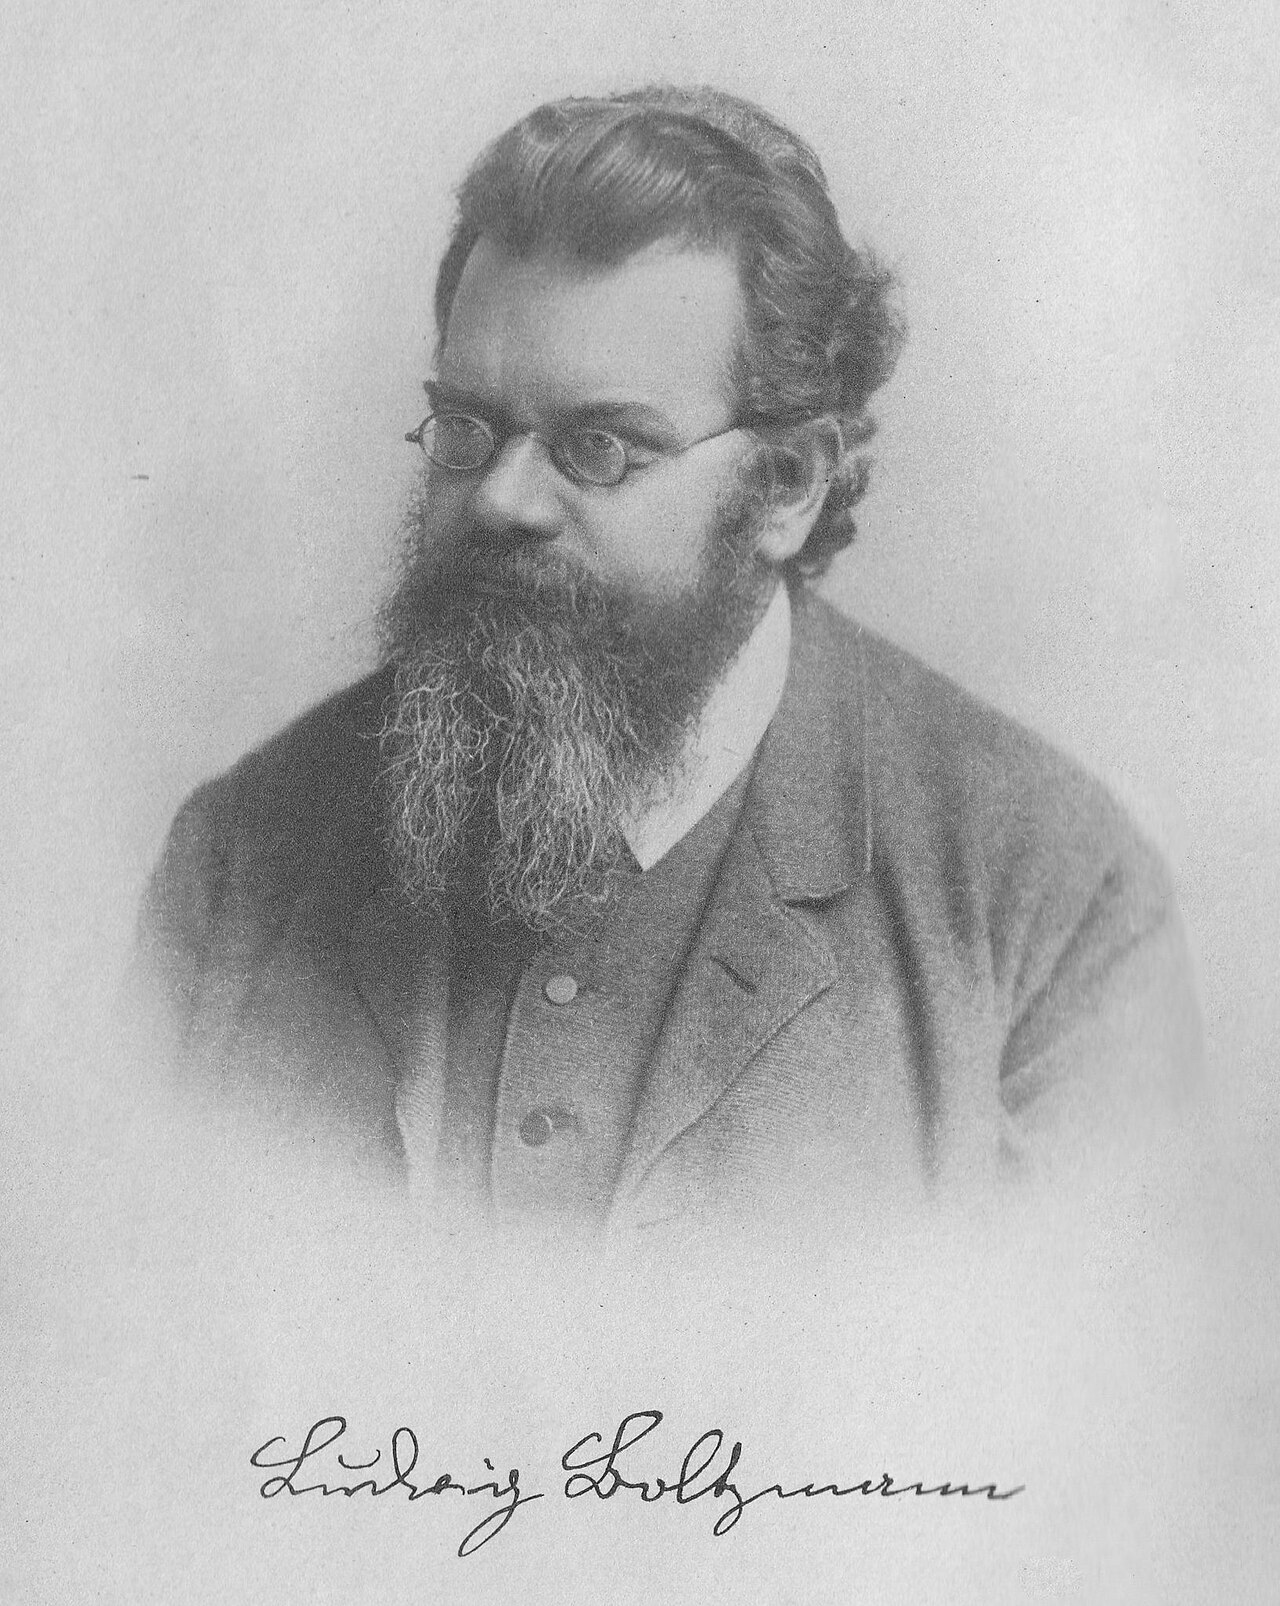
\includegraphics[width=0.3\linewidth]{images/book4/boltzmann-portrait.jpg}

{\small 路德维希·玻尔兹曼（1844--1906），其因子 $\eu^{-E/k_BT}$ 是本章的主题，其公式 $S = k_B\ln\Omega$ 刻在他位于维也纳的墓碑上。}
\end{omfigure}

\section{问题：等温大气、氦气逃逸与自旋温度计}

\begin{problem}[{周末问题——同一指数函数的三种应用}]\label{pb:b2:boltzmann-factor:1}
数据：$k_B = \qty{1.38e-23}{J/K}$，$N_A = \qty{6.02e23}{mol^{-1}}$，$g =
\qty{9.8}{m/s^2}$，$R_{\oplus} = \qty{6.37e6}{m}$，$\mu_B = \qty{9.27e-24}{J/T}$；
空气 $M = \qty{29}{g/mol}$，氦气 \qty{4}{g/mol}，氮气 \qty{28}{g/mol}。

\textbf{第一部分——等温大气。}
\begin{enumerate}
  \item 由流体静力学与理想气体定律推导 $P(z) =
        P_0\eu^{-z/H}$，并求空气在 \qty{288}{K} 时的 $H$。
  \item 指出结果中的玻尔兹曼因子，并说明是哪种能量、
        哪种温度？
  \item 求 \qty{3000}{m}、\qty{5500}{m} 和 \qty{8849}{m} 处的压强；
        以及压强减半时的高度。
  \item 求每平方米大气的质量（由 $P_0 =
        \qty{1.013e5}{Pa}$），及大气总质量；验证 $\int_0^\infty
        \rho\,\dd z = \rho_0H$。
  \item 求大气中的分子数。
  \item 若每种气体各自遵循其自身的 $H$，则
        与地面相比，\qty{50}{km} 处的 O$_2$/N$_2$ 比值将为多少？为何实际成分
        在 \qty{100}{km} 以下仍是均匀的？
  \item 真实对流层以 \qty{6.5}{K/km} 的速率降温：
        \qty{10}{km} 处的压强比等温估计值更高还是更低？
        请说明理由。
  \item 求海平面及 \qty{100}{km} 处的数密度（等温模型，
        \qty{288}{K}）；并评论“太空的边缘”。
\end{enumerate}

\textbf{第二部分——氦气逃逸。}
外逸层位于 \qty{500}{km} 以上，温度约为 \qty{1000}{K}，且
无碰撞：向上运动速率超过逃逸速率的分子
将离开大气。
\begin{enumerate}[resume]
  \item 求该高度处地球的逃逸速率。
  \item 求氦气与氮气在
        \qty{1000}{K} 时的最概然速率与平均速率。
  \item 求速率 $v > v_{\text{逃逸}}$ 的氦原子所占比例（利用
        $(2/\sqrt\pi)x\eu^{-x^2}$）；氮气同理。
  \item 逃逸氦气的通量约为 $\tfrac14n_{\text{He}}\langle
        v\rangle \times$（该比例）$\times\tfrac12$；取外逸层底部 $n_{\text{He}}
        = \qty{1e12}{m^{-3}}$，估算每平方米
        每秒及每年的损失量（针对整个地球）。
  \item 空气中氦的体积分数为 \qty{5}{ppm}：求大气中氦的总量，
        并求其相对于上述损失量的停留时间。
  \item 地壳中的放射性每年产生约 \qty{3e6}{kg} 的氦，
        大气中的氦是否处于稳态？
        与第 11 题的比较说明了什么？
  \item 太阳活动极大期间外逸层温度升至 \qty{2000}{K}：
        氦的逃逸比例将增大多少倍？
  \item 为何月球没有大气，而泰坦（逃逸速率
        \qty{2.6}{km/s}，\qty{94}{K}）却拥有厚重的大气？
\end{enumerate}

\textbf{第三部分——自旋温度计。}
某顺磁盐含有 $n = \qty{2e27}{m^{-3}}$ 个自旋 1/2，其 $\mu
= \mu_B$，置于磁场 $B$ 中。
\begin{enumerate}[resume]
  \item 求两能级的布居数及磁化强度
        $M(B,T)$。
  \item 在 $B = \qty{0.1}{T}$ 时，求 \qty{300}{K}、\qty{4}{K} 和 \qty{0.05}{K} 下的 $M$；
        居里定律在何范围内成立？
  \item 为何 $M$ 可用作温度计，它在哪个范围内最为灵敏？
        实践中测量的是什么？
  \item 求自旋的平均能量与热容（肖特基）；
        求 \qty{0.1}{T} 下热容峰值对应的温度。
  \item 求自旋在高温与零温下的熵，
        以及 $T \to 0$ 时发生了怎样的“有序化”？
  \item 由 \qty{1}{K}、\qty{1}{T} 绝热去磁至 \qty{0.01}{T}：
        求终温；为何 $B \to 0$ 时不能得到 $T \to 0$？
  \item 核自旋温度计采用 $\mu_{\text{N}} = \mu_B/1836$，在
        \qty{1}{T} 下居里定律可成立到多低的温度，
        以及为何此类温度计用于微开尔文量级？
  \item 比较谱线的多普勒展宽（由麦克斯韦分布得出）
        作为气体温度计的效用：所用的是哪个量，
        它如何随 $T$ 变化？
  \item 总结：三个体系与那一个公式。
\end{enumerate}
\end{problem}
